%% Title
%!!UPDATE THIS
\titlepage[High Energy Physics Group, Department of Physics\\ Imperial College London
]%
{\vspace*{0.6cm}
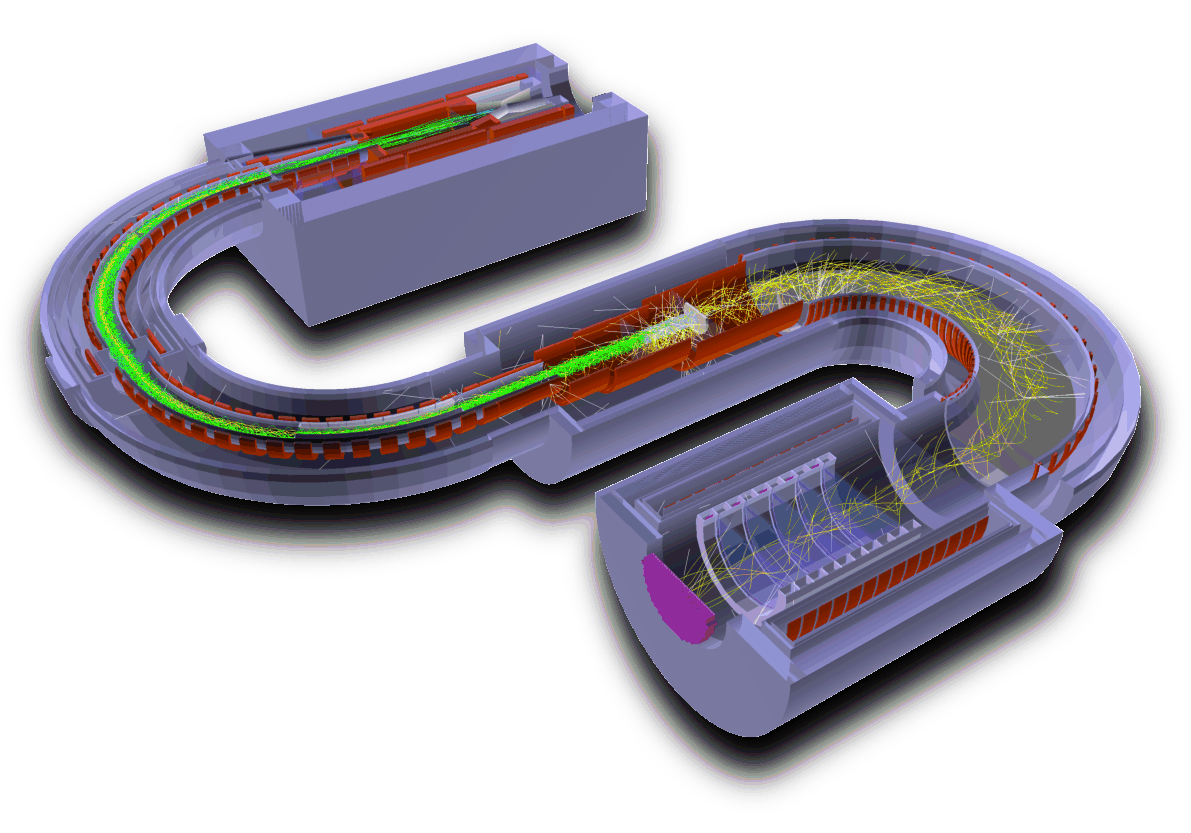
\includegraphics[width=0.9\textwidth]{figs/FrontCover_display.png}\\
\vspace*{0.7cm}
\large{A dissertation submitted to Imperial College London\\
  for the degree of Doctor of Philosophy}}
%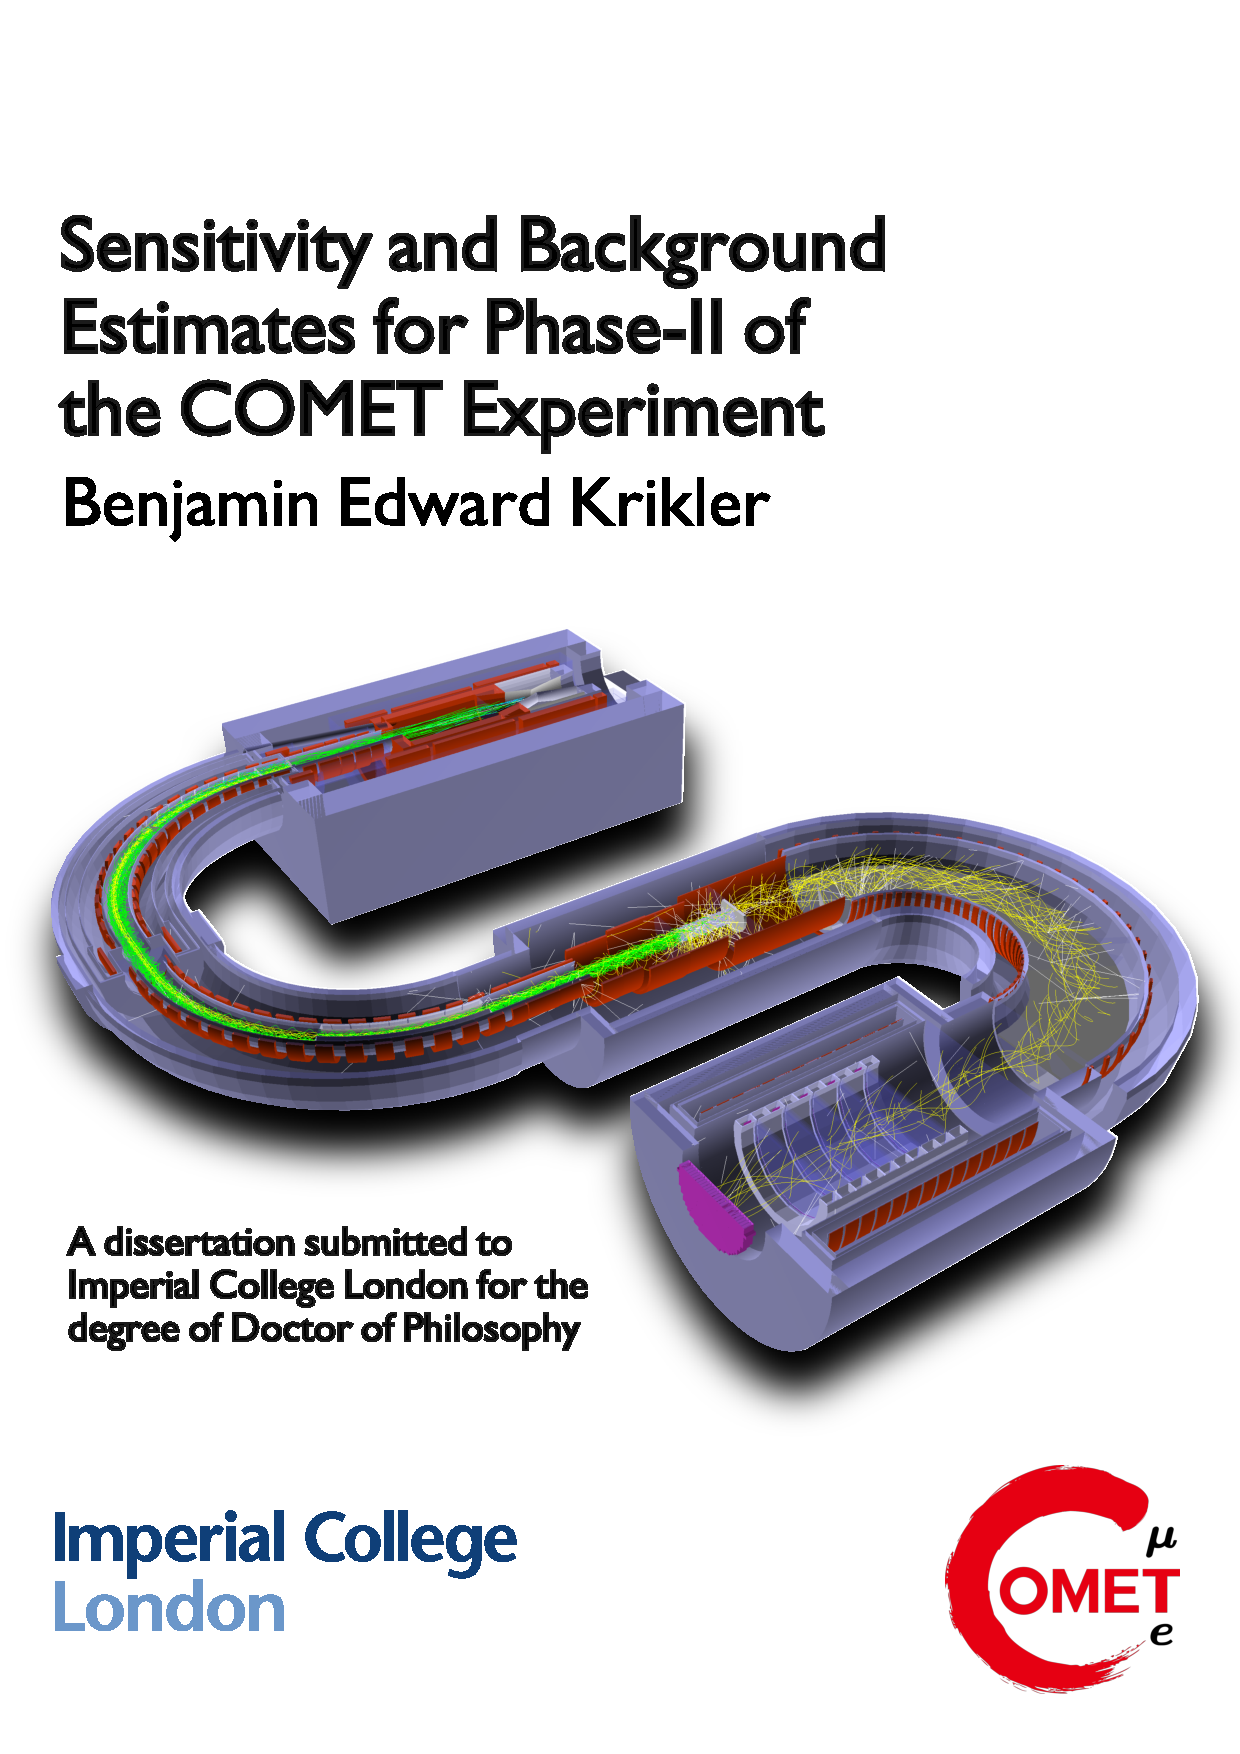
\includepdf[pages=-]{figs/FrontCover.pdf}

%% Abstract
\begin{abstract}%[\smaller \thetitle\\ \vspace*{1cm} \smaller {\theauthor}]
  %\thispagestyle{empty}
Conservation of Lepton Flavour in the Standard Model (SM) requires that neutrino emission accompanies muon decay.
COMET is one experiment looking for Charged Lepton Flavour Violation.
It searches for COherent Muon to Electron Transitions, where a muon converts to a 105~MeV electron in the presence of an atomic nucleus, without emitting neutrinos.
The current limit on this process is \senseSindrum at 90\% C.L., which COMET intends to improve by four orders of magnitude.

To realise such an improvement, COMET will use several novel techniques to produce a very intense, low-energy muon
beam, with very high signal acceptance and strong background suppression.
Given the challenge this presents, COMET will run in a staged approach.
\phaseI is currently under construction with first data-taking due in JFY 2018, and the goal of measuring \mueconv with a \ac{ses} of \sensePI.
\phaseII should follow at the start of the next decade and achieve a \ac{ses} of \sensePII.

This thesis provides an overview of CLFV, \mueconv, and the COMET experiment itself.
It sets out the software and simulation that has been developed to help understand and analyse the experiment,
and then uses this to perform a comprehensive optimisation of the \phaseII set-up, providing a new baseline configuration.
The expected performance of this baseline is assessed, with studies on the signal sensitivity
 demonstrating that an SES of \VarPredictedSES can be achieved in \VarRunTime~s of beam.
Background rates are also estimated and, although subject to large uncertainties, predict \VarTotalBgPhasII background events can be expected during \phaseII.
Suggestions for future performance studies and experiment improvements are also discussed, with a possible improvement in the SES of a factor of 2.5 likely achievable.
\end{abstract}

%% Declaration
\begin{declaration}
  This dissertation is the result of my own work, except where explicit
  reference is made to the work of others, and has not been submitted
  for another qualification to this or any other university. This
  dissertation does not exceed the word limit for the respective Degree
  Committee.
  \vspace*{0.5cm}
  \begin{flushright}
	Benjamin Edward Krikler
  \end{flushright}
  \vspace*{6cm}
The copyright of this thesis rests with the author and is made available under
a Creative Commons Attribution Non-Commercial No Derivatives licence.  Researchers
are free to copy, distribute or transmit the thesis on the condition that they
attribute it, that they do not use it for commercial purposes and that they do not
alter, transform or build upon it. For any reuse or redistribution, researchers
must make clear to others the licence terms of this work
\end{declaration}


%% Acknowledgements
\begin{acknowledgements}
Sir Isaac Newton is supposed to have said, ``If I have seen further than others it is by standing upon the shoulders of giants.''  
Exactly how tall these giants were, why they do not seem to be around any more, and how they managed to co-exist with humans, are all open questions.
One thing is certain however: if it had not been for friends, family, and colleagues, Sir Isaac would have had a much harder time getting on to the giants' shoulders.

The same has been true for my PhD, although only in the figurative sense.
Getting through the last four years would not have been possible if it were not for the people around me (none of whom are giants, sadly).

To Lorena, my brilliant fianc\'{e}e, thank you for all your support, your caring, and your patience, though I suppose I now need a new excuse beyond `PhD stress' to get out of the house work.
English may not be her first language, but that has certainly not stopped her from correcting mine.
%	has certainly not stopped her correcting my english.
%I might have spent more time in Uberlandia, Berlin, and Amsterdam, working remotely because of her, but then I did get to spend more time in Uberlandia, Berlin, and Amsterdam, working remotely.
%Thank you for all your patience, your help, your caring; I suppose I will have to find another excuse beyond thesis stress now!

Mum and dad, thank you for everything that you have given me. From the food and the chauffeuring, to the curiosity and confidence to pursue what I love, 
I can honestly say that without you, I would be less existent.
Will, Sophie, Chris, and Marie-Claire, you are all much more recent additions to my life, but it is a far better life for it; I love you all.
To my brother Dan who, ever since he was born, has been my brother---I would struggle to find a better alternative.
And to my grand-parents, my aunts, my uncles, and my cousins, and my cousins, and my cousins:  I hope I can make you all as proud of me, as I am of you.
%And then to Dan, my older younger brother.
%:And to my literally-gigantic extended family deserve a mention; I am very proud to be able to call you that.

%This PhD has been one of opportunities and variety which might not have been so, had it been focussed on any experiment but COMET.
I owe a deep gratitude to my collaborators on the COMET and AlCap experiments, who have not only endured my pedantry in code reviews, questions at collaboration meetings, and mistakes at beam tests, but they have always made me feel very welcome whilst doing it. 
%Working with collaborators from around the world has been an incredible experience in isteld.
%I have tried my best to sieze on all the opportunities you have provided me to learn and grow and mess up.
Specifically to Yoshi Kuno and Satoshi Mihara, thank you both for supporting me during my times in Japan:
I imagine few students can claim to have been personally driven to the airport by the spokesperson of their experiment!

To my COMET colleagues at Imperial, thank you too.
To my supervisor, Yoshi Uchida, not only have you pushed me to improve as a physicist, but you have also taught me the difference between an en--dash and an em---dash, and helped me to master the dark-art of that highly--complicated grammatical$-$construct that is the compound-adjective (I think).
Phill, Ewen, Per, Ajit, Peter, Jordan, Paul, Andy E.\ (previously at UCL, now at USA)---thank you all for the feedback and support you have given me over the last few years, and thank you 
	for putting up with my daft ideas and naive questions during our meetings; I am sure one day I will find a use for a reverse Monte Carlo, and I promise that you will be the first to hear!
To the rest of the Imperial HEP group, thank you too for creating such a fertile environment for a young physicist to work and grow.
Perhaps it is time to clean some of those coffee cups out now, though.

Finally, to all my friends: from home, from my undergraduate studies, from my Erasmus year, from these post-graduate studies, from Uberlandia and my trips to other places, and to all the other friends that cannot be put in a group (though I suppose that sort of defines a group):
	thank you for all the laughter, the stories, and the distractions.
It would take up too much space to write you all out in full, so I shall just put your initials here:
A, B, C, D, E, F, G, H, I, J, K, L, M, N, O, P, Q, R, S, T, U, V, W, X, Y, Z;
my apologies if I have missed anyone out!

Oh, and there is one more thank-you to make: thank you to the muon, for without you this PhD would absolutely not have been possible or else would certainly have been a lot smaller:
``The COMET experiment is searching for muon-to-electron conversion. Since there is no such thing as a muon, however, the predicted sensitivity and background rates are, respectively, zero and zero.  The end.''

%To my colleagues at Imperial, in particular, 
%To Yoshi Uchida, my supervisor, thank you for drilling home the benefits of correct latex
%The other students and the staff that I have the privilidge of being around at 
%Imperial College London has provided extremely fertile ground for me, 
%
%To my Mum and Dad, you have been 
%Unfortunately, there were few giants around for me to stand on, although I have had the gigantic support of friends, family, and colleagues, without whom I could not have managed this thesis.
%
%It is an open question as to what exactly Newton meant by this and what he was able to see.
%But just how tall were these giants, and what did they eat?  
%How did Sir Isaac get on their shoulders and where have they all gone to?
%( though, sadly, not the bit about giants).
%But just how tall were these giants, and what did they eat?  
%How did Sir Isaac get on their shoulders and where have they all gone to?
%Like many problems in physics, these are just some of the questions we still do not know.
%But if this PhD has taught me anything (which I shall leave up to my examiners to asses), it is that doing science is considerably easier when working with figurative giants.
%Perhaps, in the end, that is what Newton meant?  


\end{acknowledgements}


%% Preface
%\begin{preface}
%\end{preface}

%% ToC
\tableofcontents
\listoffigures
\listoftables

%% Strictly optional!
\frontquote%
%{Light may earth's crumbling sand be laid on thee, that dogs may dig thy bones up easily.}
%{Marcus Aurelius}
%\frontquote%
{I find it so pretentious when a thesis starts with a quote.}
{Yoshi Uchida}
%{Writing in English is the most ingenious torture\\
%   ever devised for sins committed in previous lives.}%
%  {James Joyce}
